\section{UDP protocol}

\subsection{UDP packet의 의미}
    HTTP, TCP, IP와 같은 protocol들은 각 layer에서 고유의 역할을 수행하고, 각각 다루는 data들을 layer의 기능에 따라 data에 자신의 \textbf{Header}를 붙이는 방법을 통해서 정보를 표현한다. 
    
    TCP는 packet의 전송에 있어 신뢰성과, 흐름제어, 혼잡제어등의 역할을 수행하는 protocol이기 떄문에, 각각의 Header에 기능을 수행하기 위한 값들이 포함되어 있다. \\
    \vspace{-4mm}  
        \begin{figure}[!h]\centering
    		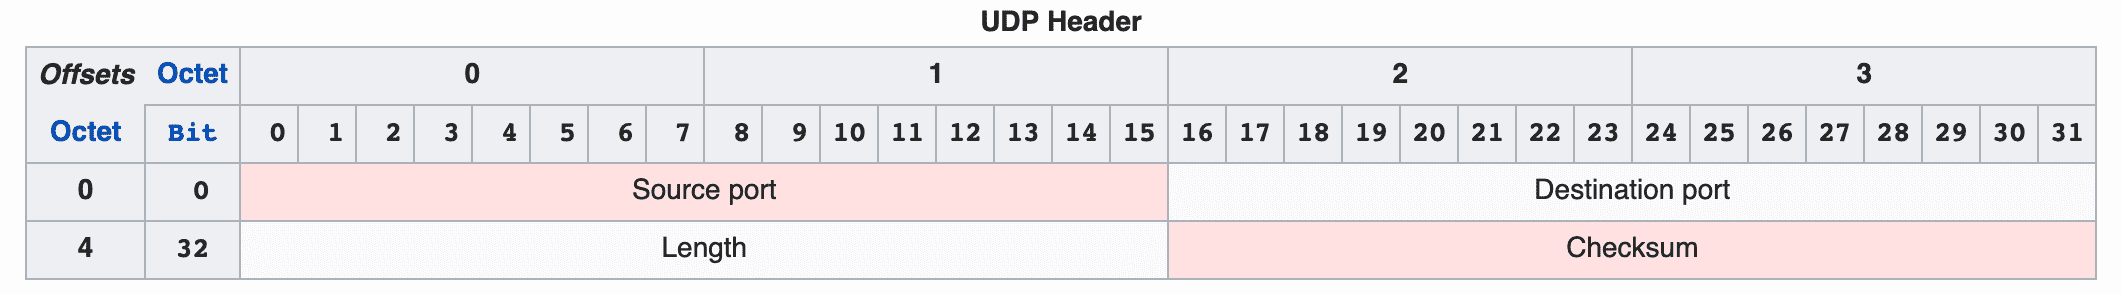
\includegraphics[width=.9\textwidth]{image/week01/2-1.png}
    		\caption{\small UDP Header}
    		\vspace{-10pt}
        \end{figure}